\documentclass{article}
    \PassOptionsToPackage{numbers, compress}{natbib}

\usepackage{neurips_2026}


\usepackage[utf8]{inputenc} % allow utf-8 input
\usepackage[T1]{fontenc}    % use 8-bit T1 fonts
\usepackage{hyperref}       % hyperlinks
\usepackage{url}            % simple URL typesetting
\usepackage{booktabs}       % professional-quality tables
\usepackage{amsfonts}       % blackboard math symbols
\usepackage{nicefrac}       % compact symbols for 1/2, etc.
\usepackage{microtype}      % microtypography
\usepackage{xcolor}         % colors

\usepackage{lmodern}
\usepackage{microtype}
\usepackage{amsmath,amssymb,amsthm,bm,mathtools}
\usepackage{booktabs}
\usepackage{graphicx}
\usepackage{xcolor}
\usepackage{enumitem}
\usepackage{multirow}
\usepackage{float}
\usepackage{hyperref}
\usepackage{cleveref}

\newcommand{\R}{\mathbb{R}}
\newcommand{\cD}{\mathcal{D}}
\newcommand{\cP}{\mathcal{P}}
\newcommand{\cE}{\mathcal{E}}
\newcommand{\cK}{\mathcal{K}}
\newcommand{\cB}{\mathcal{B}}
\newcommand{\cS}{\mathcal{S}}
\newcommand{\cU}{\mathcal{U}}
\newcommand{\vect}[1]{\boldsymbol{#1}}

% \usepackage{cite}


% Note. For the workshop paper template, both \title{} and \workshoptitle{} are required, with the former indicating the paper title shown in the title and the latter indicating the workshop title displayed in the footnote. 
\title{PathFormer: Towards a Foundation Model for Multipath Wireless Propagation}


% The \author macro works with any number of authors. There are two commands
% used to separate the names and addresses of multiple authors: \And and \AND.
%
% Using \And between authors leaves it to LaTeX to determine where to break the
% lines. Using \AND forces a line break at that point. So, if LaTeX puts 3 of 4
% authors names on the first line, and the last on the second line, try using
% \AND instead of \And before the third author name.


\author{%
  David S.~Hippocampus\thanks{Use footnote for providing further information
    about author (webpage, alternative address)---\emph{not} for acknowledging
    funding agencies.} \\
  Department of Computer Science\\
  Cranberry-Lemon University\\
  Pittsburgh, PA 15213 \\
  \texttt{hippo@cs.cranberry-lemon.edu} \\
  % examples of more authors
  % \And
  % Coauthor \\
  % Affiliation \\
  % Address \\
  % \texttt{email} \\
  % \AND
  % Coauthor \\
  % Affiliation \\
  % Address \\
  % \texttt{email} \\
  % \And
  % Coauthor \\
  % Affiliation \\
  % Address \\
  % \texttt{email} \\
  % \And
  % Coauthor \\
  % Affiliation \\
  % Address \\
  % \texttt{email} \\
}


\begin{document}


\maketitle


\begin{abstract}
  The abstract paragraph should be indented \nicefrac{1}{2}~inch (3~picas) on both the left- and right-hand margins. Use 10~point type, with a vertical spacing (leading) of 11~points. The word \textbf{Abstract} must be centered, bold, and in point size 12. Two line spaces precede the abstract. The abstract must be limited to one paragraph.
\end{abstract}

\section{Introduction}
Foundation models have reshaped artificial intelligence in text, vision, and multimodal learning by showing that broad pretraining can produce reusable backbones that transfer across many downstream tasks ~\cite{bommasani2021opportunities,brown2020language,dosovitskiy2020image,radford2021clip}.  \textbf{Emergent abilities?} In natural language processing, large language models pretrained on broad corpora now serve as general backbones for text classification, generation, and reasoning ~\cite{devlin2019bert,vaswani2017attention, guo2025deepseek}. In computer vision, and multimodal setups like vision-language and vision-language action learning, large pretrained transformers and contrastive image-text models provide similar transfer across many tasks with limited task-specific supervision \cite{pmlr-v270-kim25c, alayrac2022flamingo,  dosovitskiy2020image,radford2021clip}. The shared principle is simple: with the right pretraining object, large-scale self-supervised learning can learn representations that are reusable across different tasks. 

The wireless communication domain is another area where foundation models could thrive. This is because, as wireless signals are propagated between transmitters and receivers in different environments in the physical world, they follow the laws of Electro-Magnetic (EM) wave propagation. The propagation path of a single wave can experience complex interactions such as reflection, refraction, scattering and diffraction as it travels through different environments. These interactions become even more diverse when comparing the indoor and outdoor settings and for different weather conditions. A wireless foundation model would attempt to model this complex relationship that exists between EM wave paths and the physical environment.  In a similar way to language and vision, the foundation model with this general understanding can then be used for solving different downstream tasks in the environment. Typically, downstream tasks like channel estimation, beam prediction, user localisation, and sensing are important in optimising the communication experience between users. These tasks are even more important in 5G systems that use Millimeter-wave (mmWave) and massive multiple-input multiple-output (MIMO) systems with high data rates and fine spatial resolution, but they also impose stringent requirements on beam alignment, channel acquisition, and environment-aware inference.

Several recent works have began attempts to create these wireless foundation models. WiFo \cite{liu2025wifo} and ChannelGPT \cite{yu2024channelgpt} proposed foundation models for channel prediction and showed zero-shot generalisation for the same channel prediction task across heterogeneous Channel State Information (CSI) configurations. Large Wireless Models \cite{alikhani2024lwm} learns contextualised channel embeddings from large-scale wireless channel data and reports gains on Line of Sight (LoS) classification and beam prediction.  WirelessGPT \cite{yang2025wirelessgpt} extends the same philosophy by showing the use of the models on the downstream tasks of human activity recognition and wireless environment reconstruction. The key similarity of all these works is that they work at the channel level, with the pretraining objective been some variant of Masked Channel Modelling (MCM). This MCM is shown in Equation \ref{eq:mcm}, where the foundation model $f$ makes predictions for masked all channels positions $i \in M$, with this masking done across subcarrier, time, or space and with $h_{i}$  been the ground truth channel.

\begin{equation}
\ell_{MCM} = \frac{1}{|M|} \sum_{i \in M} || f({i|\{h_{j}\}_{j \notin M }\ }) - h_{i} ||^{2}
\label{eq:mcm}
\end{equation}




The central question, however, is whether the \emph{channel} is the right pretraining object. For a given link, the channel on subcarrier $k$ can be written as a superposition of propagation paths,
\begin{equation}
\vect{H}[k]
=
\sum_{\ell=1}^{L}
\alpha_{\ell}
\exp\!\left(-j2\pi f_k\tau_{\ell}\right)
\vect{a}_{\mathrm{rx}}\!\left(\Omega^{\mathrm{rx}}_{\ell}\right)
\vect{a}_{\mathrm{tx}}^{H}\!\left(\Omega^{\mathrm{tx}}_{\ell}\right),
\label{eq:intro_channel}
\end{equation}
where each path is characterized by a complex gain $\alpha_{\ell}$, delay $\tau_{\ell}$, and arrival/departure angles $\Omega^{\mathrm{rx}}_{\ell}$ and $\Omega^{\mathrm{tx}}_{\ell}$. Equation~\eqref{eq:intro_channel} shows the limitation of channel-level pretraining: the channel tensor mixes a variable number of path events and then further entangles them with array responses, subcarrier sampling, and system configuration. This makes it harder to isolate the environment-dependent structure that actually drives wireless behaviour. Also, users at different locations may experience a similar aggregate channel, therefore limiting the model's ability to disambiguate between the environmental signature of those users. 

We argue in this paper that a more fundamental pretraining object is the \emph{multipath process}. \emph{Path-level modeling preserves variable path cardinality, dominant-path ordering, angular structure, and interpretable physical attributes such as delay and power}. It is therefore better aligned with the idea of learning a reusable representation of wireless propagation itself rather than of one particular channel rendering. We therefore propose \emph{PathFormer}, which formulates wireless pretraining as \emph{next-path prediction} analogous to the next token prediction done in language modelling. Each transmitter-receiver pair is converted into an ordered sequence of propagation-path tokens. An autoregressive transformer is then pretrained over path sequences collected from multiple environments, in the same spirit that language models are pretrained by next-token prediction. The pretraining phase is deliberately independent of user locations; its role is to capture the general behavior of paths across different environments, not to memorize per-user coordinates. After pretraining, the backbone is adapted to target environments and reused for downstream tasks.
<< Add the problems to be answered in the modelling >>

To the best of our knowledge, PathFormer is the first wireless foundation model at the multipath level, with a formulation that represents wireless propagation as an autoregressive sequence of individual path tokens and uses \emph{next-path prediction} as the pretraining objective. A recent adjacent effort, WiCo-MG, studies multipath generation through a multipath-map representation and a different sensing-driven setup \cite{han2025wicomg}. PathFormer is instead centred on tokenized per-link path sequences and their transfer value as a reusable wireless backbone.

The main contributions of this paper are summarised below:
\begin{enumerate}[leftmargin=1.5em]
    \item We frame the need for a wireless foundation model through the same lens that has proven successful in text and show that the multipath process is a more fundamental pretraining object than the channel tensor itself. We introduce PathFormer, a path-level transformer trained with \emph{next-path prediction} and open-source the model's weights.
    \item We design a location-independent multienvironment pretraining stage whose purpose is to learn generic path behavior across environments, followed by target-environment adaptation and downstream reuse.
    \item We show that the autoregressive approach of the Pathformer outperforms non-autoregressive setups.
    \item We define and show that the pretrained PathFormer backbone can support downstream tasks such as channel user localisation, reconstruction, beam prediction, and \textbf{LoS classification}.

\end{enumerate}

\section{Literature Review}
\subsection{Existing Wireless Foundation Models}

\cite{liu2025wifo} built up on similar ideas  to \cite{alikhani2024large} in developing developing wireless channel models. However, instead of just considering an instance of time, they extend the input channels to 3D ($Time \times Freq \times Antenna$). This can the foundation model to capture temporal changes to different sub carriers frequencies and across different spatial distribution of antennas. Therefore, instead of using 2D patches, 3D patches from which masked tokens are created. Also, instead of an encoder-only architecture, a Masked-AutoEncoder \cite{he2022masked}, which has a transformer decoder in addition to the encoder, to add more capacity in the self-supervised masked reconstruction pretraining. The reconstruction tasks are now either time-masked, frequency masked or a combination of both.
\cite{yang2025wirelessgpt} proposed WirelessGPT with the goal of buidling a foundation model that extends beyond physical layer communication tasks but also to sensing tasks. The sensing downstream tasks are human activity recognition and wireless environment reconstruction. The human activity recognition involves using CSI to classify user activities such as running, walking etc. The environment reconstruction involves producing 3D point cloud representations of the environment based on the model's understanding of shadowing, scattering and reflection of rays in the environment inferred from the CSIs. 

\cite{yu2024channelgpt} introduced \textit{ChannelGPT}, a digital twin framework designed to integrate multimodal channel models into emerging 6G networks. The framework emphasized the adoption of feedback-loops both from changes to the environment and network performance to guide the operations of the channel models. Also,     the framework mentions the need of utilizing multimodal data sources, such as multi-view images of the communication environment together with channel state information (CSI), to achieve a richer and more context-aware representation of the wireless channel. The authors argue that incorporating multimodal data enables a deeper understanding of the relationship between the physical environment and the channel characteristics, thereby enhancing network performance.In contrast, other models assume that this environment and channel relationship can be implicitly learned from the variations present in the CSI data alone, without explicitly relying on multimodal inputs.
\section{Methodology}

\subsection{Background and Problem Formulation}\label{subsec:problem_formulation}
We consider a setup containing $M$ environments. For each environment $m \in \cS = \{1,\dots,M\}$, we consider the multipath propagation between transmitters (tx) $b \in \cB_m$ and receivers (rx) $u \in \cU_m$ distributed throughout the environment.  For each tx-rx pair $(m,b,u)$, we get the tx and rx positions $\vect{x}_{\mathrm{tx}}^{(m,b)}, \vect{x}_{\mathrm{rx}}^{(m,u)}  \in \R^3$, environment features $\vect{x}_{m} \in \R^{d_{env}}$,  multipath sequence $\cP_{m,b,u}$, and the corresponding channel tensor $\vect{H}_{m,b,u}$.  We show an example of such an environment in Figure \ref{fig:env_kmeans_overview}{a}.  A multipath sequence 
 with $L_{m,b,u}$ number of mulitpath is defined in Equation \ref{eqn:multpathset}. 
% $\cP_{m,b,u} \in \R^{L_{m,b,u} \times 8}$
\begin{equation}
\cP_{m,b,u} = \big(\pi^{(m,b,u)}_1,\ldots,\pi^{(m,b,u)}_{L_{m,b,u}}\big),
\label{eqn:multpathset}
\end{equation}

\begin{equation}
\pi^{(m,b,u)}_\ell = \Big(\rho_\ell, \phi_\ell, \tau_\ell, \theta^{\mathrm{aoa}}_{\ell,\mathrm{az}}, \theta^{\mathrm{aoa}}_{\ell,\mathrm{el}}, \theta^{\mathrm{aod}}_{\ell,\mathrm{az}}, \theta^{\mathrm{aod}}_{\ell,\mathrm{el}}, \vect{z}_\ell\Big).
\label{eq:path_descriptor}
\end{equation}

Each multipath $\pi^{(m,b,u)}_\ell$ component is defined in \ref{eq:path_descriptor}, where $\rho_\ell$ is the path power, $\phi_\ell$ is the phase, $\tau_\ell$ is the propagation delay, $\theta^{\mathrm{aoa}}_{\ell,\mathrm{az}}$ and $\theta^{\mathrm{aoa}}_{\ell,\mathrm{el}}$ are the azimuth and elevation angles of arrival, $\theta^{\mathrm{aod}}_{\ell,\mathrm{az}}$ and $\theta^{\mathrm{aod}}_{\ell,\mathrm{el}}$ are the corresponding angles of departure, and $\vect{z}_\ell$ is an interaction type experienced by the path. The interaction type $\vect{z}_\ell \in  \{0,1\}^4 $ is a multihot vector showing if the path experiences Reflection, Diffraction, Scattering or LoS.

\begin{figure*}[t]
    \centering
    \begin{minipage}[t]{0.49\textwidth}
        \centering
        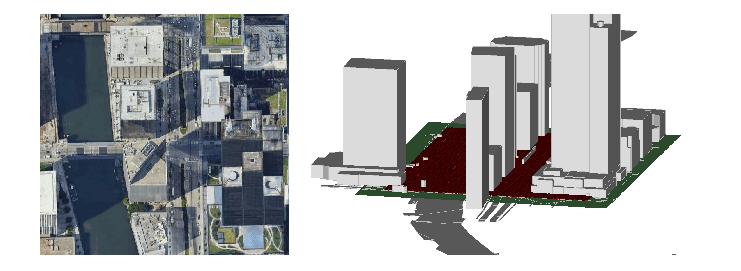
\includegraphics[height=3.0cm, width=\linewidth]{figures/user_grid_env.pdf}
        
        \vspace{2pt}
        \small \textbf{a)} Physical Environment and 3D user grid
    \end{minipage}
    \hfill
    \begin{minipage}[t]{0.49\textwidth}
        \centering
        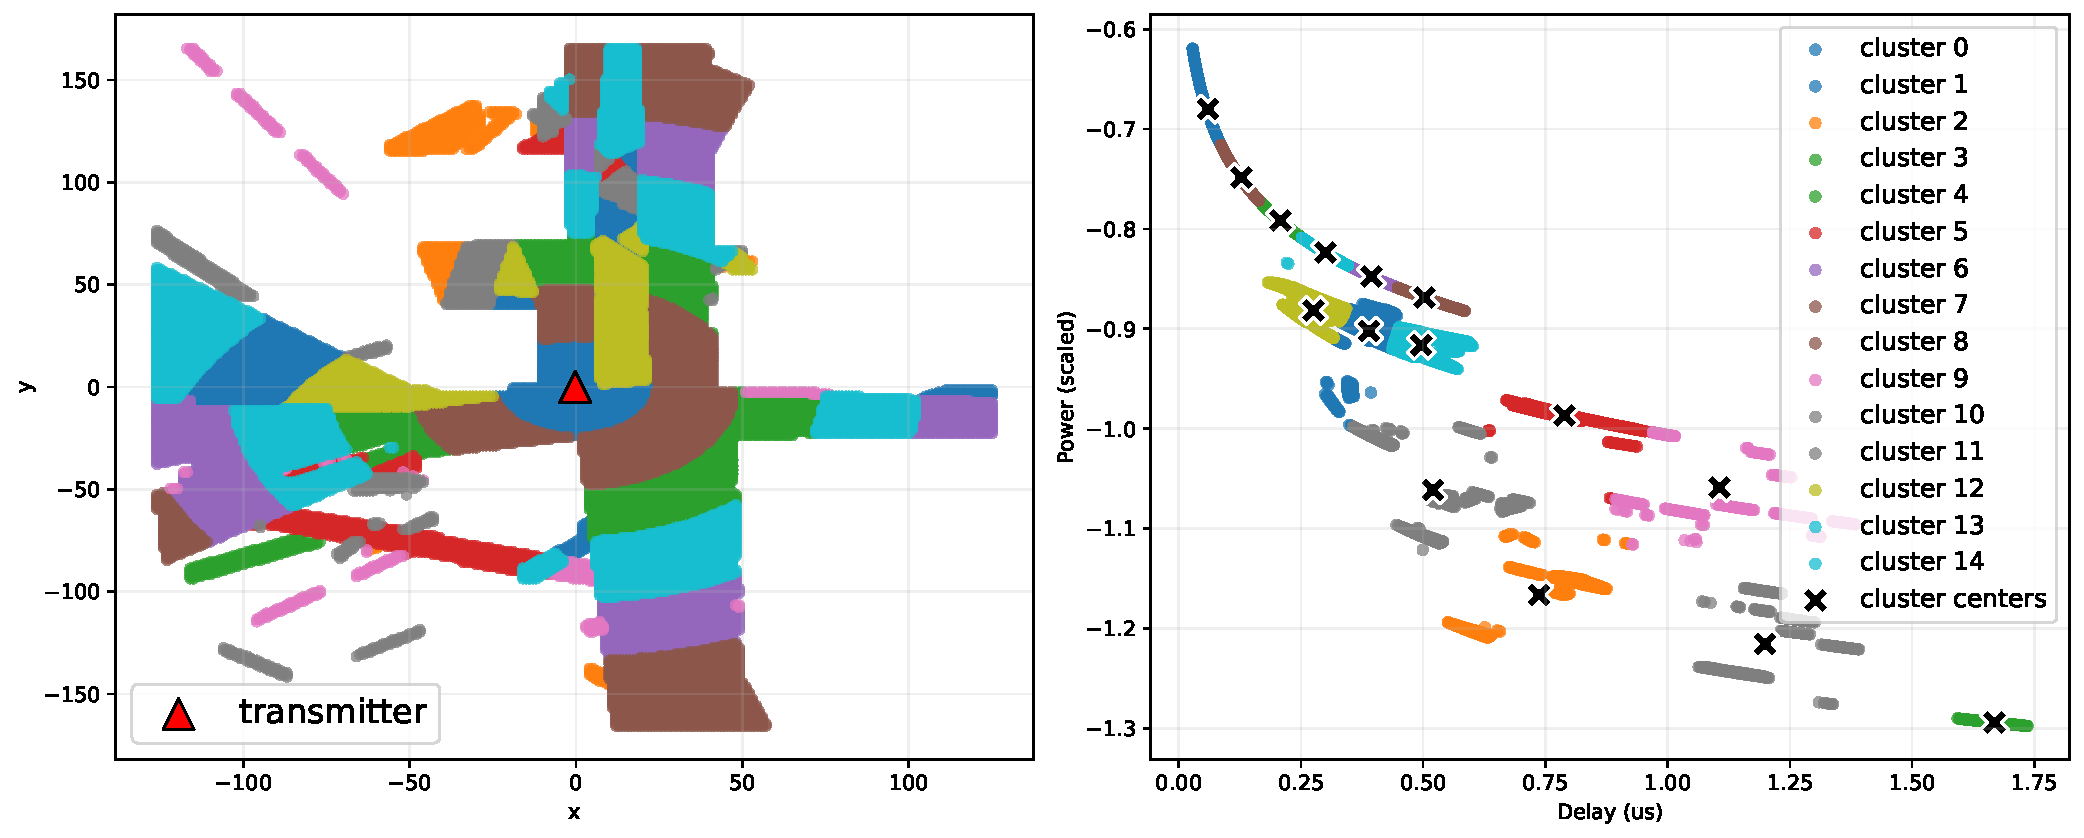
\includegraphics[height=3.0cm, width=\linewidth]{figures/first_timestep_user_kmeans.pdf}
        
        \vspace{2pt}
        \small \textbf{b)} Physical environment
    \end{minipage}
    \hfill
    \caption{
    \textbf{a)} The physical environment  and the corresponding 3D model.
    \textbf{b)} User clusters obtained from KMeans on first-path delay and power, showing that users organize into spatially coherent groups under a fixed transmitter.
    }
    \label{fig:env_kmeans_overview}
\end{figure*}

For a tx-rx pair with some features from its environment, we formulate the autoregressive modelling objective in Equation \ref{eq:next_path} to predict the arrival of the next multipath given the previous multipaths. This autoregressive formulation lends itself naturally to physical propagation because of how it closely aligns with the decay of power over subsequent paths or how paths arrive sequentially with increasing delays.

\begin{equation}
p_{\theta}(\cP_{m,n}\mid e_m)
=
\prod_{t=1}^{L_{m,n}+1}
p_{\theta}(\pi^{(m,b,u)}_t  \mid \pi^{(m,b,u)}_{<t},\vect{x}_{\mathrm{rx}}^{(m,u)}, \vect{x}_{\mathrm{tx}}^{(m,b)}, \vect{x}_{m} ).
\label{eq:next_path}
\end{equation}

This formulation leads us to \textit{solving an autoregressive variable sequence length regression problem}. This is different from the standard autoregressive formulation in language modelling for two reasons. First, in language modelling, tokens are derived from the text, yielding a vocabulary, and the model solves a \textit{variable sequence length autoregressive classification problem} over the vocabulary. Secondly, in language modelling, start and stop tokens are added to the vocabulary to initiate and terminate generation, which is not straightforward to do in a regression setup. To solve this, we first convert the path set into a deterministic ordered sequence by sorting the paths by descending power $\rho_{m,n,1} \ge \rho_{m,n,2} \ge \cdots \ge \rho_{m,n,L_{m,n}}$. The other option is to sort based on delay, because, as shown in Figure \ref{fig:env_kmeans_overview}{b}, we do not have a perfect inverse-linear relationship between received power and delay. However, we do not find any significant performance differences between the two setups. We create a start token of a vector of max power, no delays and zero angles $\pi^{(m,b,u)}_0 ={\textbf{0}}$ to initiate generation. At each timestep, the model simulatenously predicts the path parameters defined in Equation \ref{eq:path_descriptor}.  To terminate generation, rather than define a target end-of-sentence path, which could hurt the performance in a regression setup, we explicitly predict the number of paths between the transmitter and receiver and use that to terminate. Analogously to how Retrieval Augmented Generation (RAG) has helped to augment language prompts with relevant context, we propose an \textit{Environmental RAG framework }in section \ref{subsec:env_rag} on how to extract the relevant environmental features $\vect{x}_{m}$ relevant to the tx-rx pair. 
\subsection{PathFormer Backbone Model}
We propose to solve the problem formulated in \ref{eq:next_path} with our Pathformer Model. The Pathformer model uses an encoder-decoder transformer architecture similar to Vision Language Models\cite{li2023trocr,alayrac2022flamingo}, with the encoder and decoder capturing information from different modalities.  The encoder produces representations capturing the relationship between tx-rx and the physical environment. To encourage the encoder to produce environmentally grounded representations and also to solve the variable sequence length introduced in Section \ref{subsec:problem_formulation}, we supervise the encoder's representation to be predictive of the number of multipaths between the tx-rx. The decoder then captures how the current path relates to previous paths conditioned on the environment encoder's representations. Therefore, the encoder works in the physical environment modality, and the decoder primarily works in the EM multipath modality. This process in the pathformer to produce the hidden state at generation step $t$ is captured in Equation \ref{eq:backbone}. 
\begin{figure}
    \centering
    \fbox{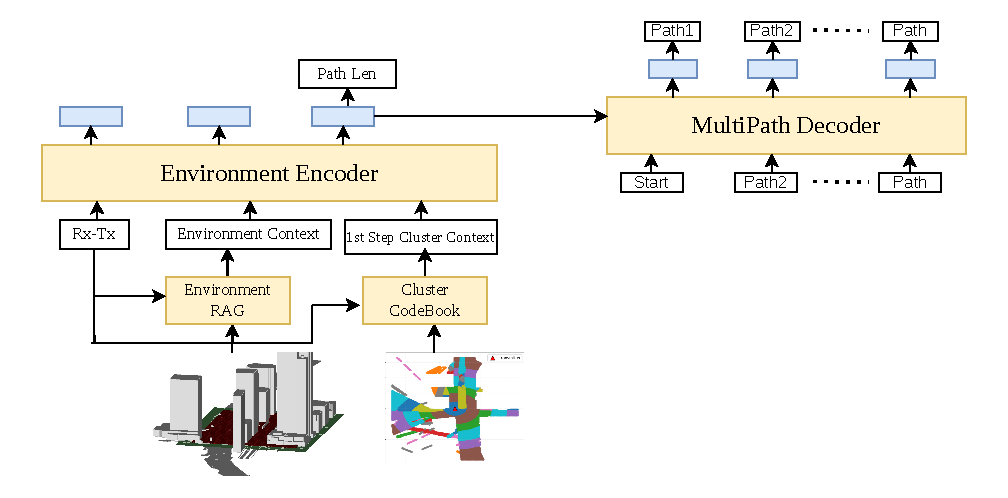
\includegraphics[width=\linewidth]{figures/PathFormer-Page-7.drawio.pdf}}
    \caption{
    Overview of the proposed corridor-aware PathFormer. The model augments the tx-rx prompt with Environmental RAG features and a first-path KMeans codebook, then autoregressively predicts the multipath sequence with a residual correction for the dominant first path.
    }
    \label{fig:pathformer_corridor}
\end{figure}

\begin{equation}
\vect{E}_{env}
=
\mathrm{Encoder}_{\theta}( [x_m, x_{tx}, x_{rx}] )
\label{eq:backbone}
\end{equation}

\begin{equation}
\hat{L}_{m,b,u}
=
f_{\mathrm{len}}(\vect{E}_{\mathrm{env}}),
\label{eq:pathformer_length_head}
\end{equation}

\begin{equation}
\vect{h}_t
=
\mathrm{Decoder}_{\theta}
\Big(
[\vect{E}_{env};\,E_{\mathrm{tok}}(o_{<t}) + \vect{p}_{<t}]
\Big),
\label{eq:backbone}
\end{equation}
From $\vect{h}_t$, the model predicts the next path token $\widehat{\vect{y}}_t$ including the interactions experienced  $\hat{\vect{z}}_t \in [0,1]^4$ using Equations \ref{eq:pathformer_reg_head} and \ref{eq:pathformer_interaction_head}. Each element in $\hat{\vect{z}}_t$ is the corresponding probabilities for the interaction labels. This is because a path may simultaneously experience multiple interaction types (e.g. reflection and refraction), predicting $\vect{z}_t$ is a \emph{multilabel classification problem} with its loss defined in Equation \ref{eq:interaction_loss}.
\begin{equation}
\widehat{\vect{y}}_t =
\Big(
\hat{\tau}_t,\hat{\rho}_t,
\widehat{\sin\phi_t},\widehat{\cos\phi_t},
\widehat{\sin\theta^{\mathrm{aoa}}_{t,\mathrm{az}}},\widehat{\cos\theta^{\mathrm{aod}}_{t,\mathrm{az}}},
\widehat{\sin\theta^{\mathrm{aoa}}_{t,\mathrm{el}}},\widehat{\cos\theta^{\mathrm{aod}}_{t,\mathrm{el}}}
\Big)
=
W_{\mathrm{reg}}\vect{h}_t + \vect{b}_{\mathrm{reg}},
\label{eq:pathformer_reg_head}
\end{equation}

\begin{equation}
\vect{s}_t
=
W_{\mathrm{int}}\vect{h}_t + \vect{b}_{\mathrm{int}},
\qquad
\hat{\vect{z}}_t = \sigma(\vect{s}_t),
\label{eq:pathformer_interaction_head}
\end{equation}
For a path with length $L_{m,b,u}$ We compute an L2 loss for the other parameters and the path length in (Equations \ref{eq:path_l2_loss_transformed} and \ref{eq:path_length_loss}). We define total loss as a weighted combination of these three objectives in Equation \ref{eq:total_loss}.

\begin{equation}
\mathcal{L}_{\mathrm{path}}
=
\frac{1}{L_{m,b,u}}
\sum_{t}
\left\|
\hat{\vect{y}}_t-\vect{y}_t
\right\|_2^2,
\label{eq:path_l2_loss_transformed}
\end{equation}

\begin{equation}
\mathcal{L}_{\mathrm{len}}
=
\left(
\hat{L}_{m,b,u}-L_{m,b,u}
\right)^2,
\label{eq:path_length_loss}
\end{equation}


\begin{equation}
\mathcal{L}_{\mathrm{int}}
=
\frac{1}{L_{m,b,u}}
\sum_{t}\sum_{k=1}^{4}
\left[
-z_{t,k}\log \sigma(s_{t,k})
-(1-z_{t,k})\log\big(1-\sigma(s_{t,k})\big)
\right],
\label{eq:interaction_loss}
\end{equation}

\begin{equation}
\mathcal{L}
=
\mathcal{L}_{\mathrm{path}}
+
\lambda_{\mathrm{int}}\mathcal{L}_{\mathrm{int}}
+
\lambda_{len}\mathcal{L}_{len}
\label{eq:total_loss}
\end{equation}

\subsection{Environmental Retrieval Augmented Generation}
\label{subsec:env_rag}

During propagation, multipaths interact with a variety and density of objects in the environment. Environments can vary starkly, with sparser buildings in less populated areas to more dense objects and users in urban settings. We, however, require our model to be able to reason about relevant objects in all types of environments in an efficient manner.
The naive approach of passing a single global environment descriptor $\vect{x}_m$ may be too coarse, noisy and inefficient for path prediction for disambiguating users across different varying environments. The paths for a tx-rx pair are determined not only by which environment the pair belongs to, but more specifically by \emph{which objects are locally close to the receiver and which objects lie along the tx-rx propagation corridor}. This motivates our \emph{Environmental Retrieval RAG} framework, which retrieves tx-rx-specific geometric context from the scene and conditions the Pathformer on this retrieved representation. We consider an environment $m$, with tx-rx pair located at $\vect{p}^{(m,b)}_{\mathrm{tx}}, \vect{p}^{(m,u)}_{\mathrm{rx}} \in \mathbb{R}^2$, with   $\mathcal{O}_m=\{o^{(m)}_1,\dots,o^{(m)}_{J_m}\}$
denoting the set of physical objects in the scene. Each object $o^{(m)}_j$ is associated with geometric attributes such as planar centroid $\vect{p}^{(m)}_j\in\mathbb{R}^2$, height $h^{(m)}_j$, footprint area $a^{(m)}_j$, and material properties.

\paragraph{Local dense retrieval.}
For a query point $\vect{q}\in\mathbb{R}^2$ and radius $d_{\max}$, we define the local object candidate set in Equation \ref{eq:candidate_set} and retain the $K$ nearest objects \ref{eq:local_retrieval}.
\begin{equation}
\mathcal{O}_{m}(\vect{q}, d_{\max})
=
\left\{
o_j \in \mathcal{O}_m :
\left\|
\vect{p}^{(m)}_j-\vect{q}
\right\|_2 \le d_{\max}
\right\},
\label{eq:candidate_set}
\end{equation}

\begin{equation}
\mathcal{N}_{K}(\vect{q}, d_{\max})
=
\operatorname{TopK}_{o_j \in \mathcal{O}_{m}(\vect{q}, d_{\max})}
\left\|
\vect{p}^{(m)}_j-\vect{q}
\right\|_2 .
\label{eq:local_retrieval}
\end{equation}
We apply this retrieval at both $\vect{q}=\vect{p}^{(m,u)}_{\mathrm{rx}}$ and $\vect{q}=\vect{p}^{(m,b)}_{\mathrm{tx}}$. For each retrieved object, we keep a dense description consisting of distance, height, footprint area, and material properties. 



\paragraph{Corridor dense retrieval.}
To capture objects that are not close to either endpoint but still lie near the propagation route, we define a tx-rx corridor. For each object $o_j$ with its centroid at $p_{j}$, we project it onto the tx-rx line using Equation \ref{eq:corridor_segment} and then compute the distance of the object to that point on the tx-rx line segment in Equation \ref{eq:corridor_distance}. Finally, we then retrieve Top-k close objects in a similar manner to Equation \ref{eq:local_retrieval}.
% \begin{equation}
% \mathcal{C}_{m,b,u}(j)
% =
% \vect{p}^{(m,b)}_{\mathrm{tx}}
% +
% \alpha_j
% \big(\vect{p}^{(m,u)}_{\mathrm{rx}}-\vect{p}^{(m,b)}_{\mathrm{tx}}\big),
% \label{eq:corridor_segment}
% \end{equation}
% where
% \begin{equation}
% \alpha_j
% =
% \frac{
% (\vect{p}^{(m)}_j-\vect{p}^{(m,b)}_{\mathrm{tx}})^\top
% (\vect{p}^{(m,u)}_{\mathrm{rx}}-\vect{p}^{(m,b)}_{\mathrm{tx}})
% }{
% \left\|
% \vect{p}^{(m,u)}_{\mathrm{rx}}-\vect{p}^{(m,b)}_{\mathrm{tx}}
% \right\|_2^2
% }.
% \label{eq:projection_coeff}
% \end{equation}

\begin{equation}
\mathcal{C}_{m,b,u}(j)
=
\vect{p}^{(m,b)}_{\mathrm{tx}}
+
\text{proj}_{\mathbf{\vect{p}^{(m,u)}_{\mathrm{rx}}-\vect{p}^{(m,b)}_{\mathrm{tx}}}} (\vect{p}^{(m)}_j-\vect{p}^{(m,b)}_{\mathrm{tx}} )
\label{eq:corridor_segment}
\end{equation}

\begin{equation}
d^{\mathrm{cor}}_j
=
\left\|
\vect{p}^{(m)}_j-\mathcal{C}_{m,b,u}(j)
\right\|_2.
\label{eq:corridor_distance}
\end{equation}

% In practice, we clip $\alpha_j$ to $[0,1]$ so that $\mathcal{C}_{m,b,u}(j)$ lies on the finite transmitter--receiver segment rather than on its infinite line extension. We then retain the $K$ closest objects within corridor radius $d_{\max}$:
% \begin{equation}
% \mathcal{N}^{\mathrm{cor}}_{K}(d_{\max})
% =
% \operatorname{TopK}_{o_j \in \mathcal{O}_m:\, d^{\mathrm{cor}}_j \le d_{\max}}
% d^{\mathrm{cor}}_j .
% \label{eq:corridor_retrieval}
% \end{equation}


\paragraph{Sparse multi-scale summaries.}
The dense top-$K$ retrieval captures the most relevant individual objects but not the broader spatial distribution of clutter. Moreover, we need to capture to capture some summarised information about objects within $d_{max}$ but not captured in the top-$K$.  We therefore add sparse summaries computed over increasing radii $\{d_1,\dots,d_R\}$.  Around both the transmitter and receiver, we compute object counts and maximum object heights within each radius. Similarly, around the tx-rx corridor, we partition the tx-rx segment into $B$ bins and, within corridor radius $d_{\max}$, compute per-bin summaries of object count and maximum height. These sparse features provide a coarse multi-scale description of environmental density and obstruction patterns. We concatenate the local, dense, and sparse summaries around to have our full retrieval context.
\begin{equation}
\vect{r}_{m,b,u}
=
\psi\!\Big(
\mathcal{N}_{K}(\vect{p}^{(m,u)}_{\mathrm{rx}}, d_{\max}),
\mathcal{N}_{K}(\vect{p}^{(m,b)}_{\mathrm{tx}}, d_{\max}),
\mathcal{N}^{\mathrm{cor}}_{K}(d_{\max})
\Big),
\label{eq:retrieval_vector}
\end{equation}
where $\psi(\cdot)$ concatenates: (i) dense features for the top-$K$ local objects around the receiver and transmitter, (ii) dense features for the top-$K$ objects nearest to the transmitter--receiver corridor, and (iii) sparse multi-scale summaries over local radii and corridor bins. This representation is both efficient and pair-specific: the dense component preserves the most relevant object-level information, while the sparse component captures broader environmental structure.


\paragraph{First-Path Cluster CodeBook.}
Because the path sequence is sorted by descending power, the first path often corresponds to the dominant propagation mode. Empirically, this first path exhibits strong spatial regularity: nearby users served by the same transmitter often share similar first-path delay and power. We exploit this structure by learning a transmitter-specific KMeans prior over the first-path target
\begin{equation}
\vect{y}^{(1)}_{m,b,u}
=
\begin{bmatrix}
\tau_1^{(m,b,u)}\\
\rho_1^{(m,b,u)}
\end{bmatrix}.
\label{eq:first_path_target}
\end{equation}

For each transmitter $b$ in environment $m$, we fit KMeans on the training set:
\begin{equation}
\{\vect{c}^{(m,b)}_k\}_{k=1}^{K}
=
\mathrm{KMeans}\!\left(
\{\vect{y}^{(1)}_{m,b,u}:u\in\mathcal{U}^{\mathrm{train}}_m\}
\right),
\label{eq:kmeans_centers}
\end{equation}
where $\vect{c}^{(m,b)}_k\in\mathbb{R}^2$ is the $k$-th cluster centroid. We also compute the within-cluster dispersion
\begin{equation}
\vect{\sigma}^{(m,b)}_k
=
\mathrm{Std}\!\left(
\{\vect{y}^{(1)}_{m,b,u}: z^{(m,b,u)}=k\}
\right),
\label{eq:kmeans_std}
\end{equation}
where $z^{(m,b,u)}$ is the cluster assignment.

At test time, a receiver is assigned a first-path prior through nearest-neighbor transfer within the same transmitter:
\begin{equation}
u^\star
=
\arg\min_{u' \in \mathcal{U}^{\mathrm{train}}_m(b)}
\left\|
\vect{x}^{(m,u)}_{\mathrm{rx}}
-
\vect{x}^{(m,u')}_{\mathrm{rx}}
\right\|_2^2,
\label{eq:nn_assignment}
\end{equation}
and the corresponding cluster prior is
\begin{equation}
\vect{c}_{m,b,u}=\vect{c}^{(m,b)}_{z^{(m,b,u^\star)}},
\qquad
\vect{\sigma}_{m,b,u}=\vect{\sigma}^{(m,b)}_{z^{(m,b,u^\star)}}.
\label{eq:assigned_cluster_prior}
\end{equation}

\paragraph{Residual First-Path Prediction.}
We use the KMeans centroid as a strong initialization for the first path, and train the model to predict only the residual correction:
\begin{equation}
\widehat{\vect{y}}^{(1)}_{m,b,u}
=
\vect{c}_{m,b,u}
+
f_{\mathrm{res}}
\Big(
\vect{h}_1,\,
\vect{c}_{m,b,u},\,
\vect{\sigma}_{m,b,u},\
\vect{r}_{m,b,u}
\Big),
\label{eq:first_path_residual}
\end{equation}
where $\vect{h}_1$ is the decoder hidden state at the first generation step. This design is important: the KMeans prior captures a strong spatial mode for the dominant path, while the residual term allows the network to adapt that prior using the retrieved environmental geometry. In other words, KMeans provides a robust default hypothesis, and Environmental RAG provides the scene evidence needed to refine it. For subsequent paths $t\geq 2$, the model reverts to the standard autoregressive prediction defined by the PathFormer decoder. Thus, the full framework combines:
(i) retrieval of tx-rx pair-specific environmental context,
(ii) a cluster codebook prior for the dominant path, and
(iii) autoregressive sequence modeling for the remaining multipath components.

% \paragraph{Intuition.}
% The proposed Environmental RAG framework addresses two limitations of using only a coarse environment embedding. First, local receiver-side features alone cannot explain dominant blockers or reflectors that lie far from the receiver but directly along the propagation route. Second, learning the first path entirely from scratch forces the network to rediscover a strong low-dimensional spatial prior that can be estimated much more reliably with a simple clustering model. By combining corridor-aware retrieval with a KMeans-based first-path prior, the model receives both \emph{geometric scene evidence} and a \emph{strong dominant-path initialization}, leading to more stable and physically grounded predictions.


\subsection{Multi-Environment Pretraining and Finetuning}\label{sec:pretrain_finetune}
% Since multipath propagation exhibits both environment-specific structure and cross-environment regularities, we adopt a two-stage training strategy. First, we pretrain PathFormer jointly across multiple environments so that it learns general sequential regularities of multipath generation. We then finetune the pretrained backbone on a target environment, where the transmitter and receiver geometry is provided explicitly. During multi-environment pretraining (Equation \ref{eq:pretraining}), we mask the transmitter and receiver locations so that the model cannot rely on user-specific geometry and must instead capture environment-level and sequence-level propagation patterns.
% \begin{equation}
% \vect{E}_{env}^{\mathrm{pre}}
% =
% \mathrm{Encoder}_{\theta}\big([\,\vect{x}_m,\vect{0}_{tx},\vect{0}_{rx}\,]\big).
% \label{eq:pretraining}
% \end{equation}
% The foundation model here is optimised over samples drawn from all training environments on the objective in Equation \ref{eq:total_loss}. In this way, the model learns a user-agnostic foundation prior over multipath sequences. After pretraining, the model is adapted to a target environment by restoring the transmitter and receiver locations:
% \begin{equation}
% \vect{E}_{env}^{\mathrm{ft}}
% =
% \mathrm{Encoder}_{\theta}\big([\,\vect{x}_m,\vect{x}_{tx},\vect{x}_{rx}\,]\big).
% \label{eq:finetuning}
% \end{equation}
% Starting from the pretrained parameters $\theta_{\mathrm{pre}}$, we finetune the model on environment-specific samples to obtain
% \begin{equation}
% \theta_{\mathrm{ft}}
% =
% \arg\min_{\theta}
% \mathbb{E}_{(m,b,u)\sim \mathcal{D}_{\mathrm{target}}}
% \left[
% \mathcal{L}_{\mathrm{path}}
% +
% \lambda_{\mathrm{len}}\mathcal{L}_{\mathrm{len}}
% +
% \lambda_{\mathrm{int}}\mathcal{L}_{\mathrm{int}}
% \right].
% \label{eq:finetune_loss}
% \end{equation}
% This stage adapts the general sequential prior learned during pretraining to the geometry and propagation dynamics of the target environment.

\subsection{Downstream Task Reuse}\label{sec:down}
We describe how the foundation model can be used for the downstream tasks, both in \emph{zero-shot style and adapter finetuning}. We consider the tasks of \textit{beam prediction, user-localisation, and channel estimation}. 
For the adapter fine-tuning, we freeze the backbone Pathformer model and finetune some MLP heads for some downstream tasks. This leverages the generalised representations from the pathformer backbone and allows for efficient finetuning of few parameters from the added MLP heads. We apply a pool function (e.g. mean, first) to the hidden representation produced during autoregressive rollout as shown in Equation \ref{eq:pool}. 

\begin{equation}
\bar{\vect{h}}_{m,n} = \Pool\big(\vect{h}_1,\ldots,\vect{h}_{\hat{L}_{m,n}}\big)
\label{eq:pool}
\end{equation}


\paragraph{Channel reconstruction.}
The predicted path sequence can be rendered back into a channel estimate using the same physical model,
\begin{equation}
\hat{\vect{H}}_{m,n}[k]
=
\sum_{t=1}^{\hat{L}_{m,n}}
\hat{\alpha}_{m,n,t}
\exp\!\left(-j2\pi f_k\hat{\tau}_{m,n,t}\right)
\vect{a}_{\mathrm{rx}}\!\left(\hat{\theta}^{\mathrm{aoa}}_{m,n,t,\mathrm{az}},\hat{\theta}^{\mathrm{aoa}}_{m,n,t,\mathrm{el}}\right).
\label{eq:channel_reconstruction}
\end{equation}
The resulting channel can be evaluated using
\begin{equation}
\NMSE
=
\frac{\sum_{k \in \cK}\|\hat{\vect{H}}[k]-\vect{H}[k]\|_F^2}
{\sum_{k \in \cK}\|\vect{H}[k]\|_F^2}.
\label{eq:nmse}
\end{equation}

\paragraph{Beam prediction}
Given a beam codebook $\mathcal{W}=\{\vect{w}_1,\ldots,\vect{w}_{|\mathcal{W}|}\}$, beam selection from the reconstructed channel can be written as
\begin{equation}
\hat{b}_{m,n}
=
\arg\max_{q \in \{1,\ldots,|\mathcal{W}|\}}
\sum_{k \in \cK}
\left\|\vect{w}_q^{H}\hat{\vect{H}}_{m,n}[k]\right\|_2^2.
\label{eq:beam_selection}
\end{equation}
A lightweight classifier head on $\bar{\vect{h}}_{m,n}$ can also be used if desired.

\paragraph{User Localization.}
For user localization, a regression head is attached to the pooled hidden state,
\begin{equation}
\hat{\vect{x}}^{\mathrm{rx}}_{m,n} = f_{\mathrm{loc}}(\bar{\vect{h}}_{m,n}).
\label{eq:localization}
\end{equation}
This evaluates whether the pretrained backbone captures information that is useful not only for forward channel synthesis but also for inverse geometric inference.
\section{Experiments}
\subsection{Datasets}


We evaluate our method using the DeepMIMO dataset framework \cite{DBLP:journals/corr/abs-1902-06435}, which provides site-specific wireless datasets derived from ray-tracing simulations. DeepMIMO is especially well suited to our setting because it exposes not only channel responses, but also the geometric and path-level propagation structure underlying those channels. In particular, the framework supports the generation and storage of transmitter-receiver geometry, path interactions, and channel realizations in a unified format, which aligns naturally with our formulation of multipath propagation as a sequential prediction problem.  A key advantage of DeepMIMO is that it acts as a bridge between ray tracers and wireless simulation pipelines. The current DeepMIMO toolchain supports integration with NVIDIA Sionna RT \cite{hoydis2023sionnaopensourcelibrarynextgeneration}, Remcom Wireless InSite \cite{remcom}, Nvidia AODT \cite{aodt} and other ray-tracing sources through standardised conversion and dataset-generation utilities. This makes it possible to construct realistic, reproducible, and shareable datasets across a wide range of environments while preserving the physical propagation information needed for learning-based channel modelling.



It is worth noting that DeepMIMO is fundamentally a ray-tracing-based dataset framework rather than a native real-world measurement dataset. In other words, the datasets are generated from high-fidelity propagation simulations and converted ray-tracing outputs, rather than being primarily collections of measured over-the-air channel data. This makes DeepMIMO particularly valuable for controlled and reproducible benchmarking, though it should be interpreted as a physically grounded simulation benchmark rather than a purely measurement-driven one.


\begin{table}[t]
\centering
\caption{Cross-scenario MAE comparison over 32 scenarios.}
\label{tab:main_mae_results}
% \scriptsize
\resizebox{\columnwidth}{!}{%
\begin{tabular}{lcccccccc}
\toprule
Model & Delay & Power & AoA Az & AoA El & AoD Az & AoD El & Int. Acc. & Int. F1 \\
\midrule
Direct & 0.108 $\pm$ 0.075 & 7.346 $\pm$ 3.879 & 32.142 $\pm$ 23.252 & 4.766 $\pm$ 4.287 & 31.002 $\pm$ 21.519 & 3.934 $\pm$ 3.373 & 0.874 $\pm$ 0.069 & 0.792 $\pm$ 0.201 \\
Residual & 0.088 $\pm$ 0.062 & 4.294 $\pm$ 3.051 & 29.556 $\pm$ 21.950 & 4.790 $\pm$ 4.251 & 28.842 $\pm$ 20.120 & 3.775 $\pm$ 3.305 & 0.902 $\pm$ 0.063 & 0.845 $\pm$ 0.172 \\
Corridor & \textbf{0.068} $\pm$ \textbf{0.054} & \textbf{3.262} $\pm$ \textbf{2.857} & \textbf{23.099} $\pm$ \textbf{20.916} & \textbf{3.806} $\pm$ \textbf{3.458} & \textbf{21.390} $\pm$ \textbf{19.742} & \textbf{3.155} $\pm$ \textbf{2.840} & \textbf{0.928} $\pm$ \textbf{0.059} & \textbf{0.896} $\pm$ \textbf{0.143} \\
\bottomrule
\end{tabular}
}
\end{table}








{
\small
\bibliographystyle{unsrt}
\bibliography{references}
}
% \section*{References}


% References follow the acknowledgments in the camera-ready paper. Use unnumbered first-level heading for
% the references. Any choice of citation style is acceptable as long as you are
% consistent. It is permissible to reduce the font size to \verb+small+ (9 point)
% when listing the references.
% Note that the Reference section does not count towards the page limit.
% \medskip


% {
% \small


% [1] Alexander, J.A.\ \& Mozer, M.C.\ (1995) Template-based algorithms for
% connectionist rule extraction. In G.\ Tesauro, D.S.\ Touretzky and T.K.\ Leen
% (eds.), {\it Advances in Neural Information Processing Systems 7},
% pp.\ 609--616. Cambridge, MA: MIT Press.


% [2] Bower, J.M.\ \& Beeman, D.\ (1995) {\it The Book of GENESIS: Exploring
%   Realistic Neural Models with the GEneral NEural SImulation System.}  New York:
% TELOS/Springer--Verlag.


% [3] Hasselmo, M.E., Schnell, E.\ \& Barkai, E.\ (1995) Dynamics of learning and
% recall at excitatory recurrent synapses and cholinergic modulation in rat
% hippocampal region CA3. {\it Journal of Neuroscience} {\bf 15}(7):5249-5262.
% }


%%%%%%%%%%%%%%%%%%%%%%%%%%%%%%%%%%%%%%%%%%%%%%%%%%%%%%%%%%%%

\appendix

\section{Additional Model and Training Details}
\label{appendix:model_training}

This appendix summarizes the model configurations and training settings used in our experiments. All models operate on path tokens of the form
\(
[\tau,\rho,\phi,\theta^{\mathrm{aoa}}_{\mathrm{az}},\theta^{\mathrm{aoa}}_{\mathrm{el}},\theta^{\mathrm{aod}}_{\mathrm{az}},\theta^{\mathrm{aod}}_{\mathrm{el}}]
\)
and predict a multi-label interaction vector for each path. We use a zero-valued start token, sort paths by descending received power, and predict the path count with a dedicated length head to terminate generation.

\begin{table}[h]
\centering
\caption{Summary of the three model configurations used in the main experiments.}
\label{tab:appendix_model_configs}
\small
\begin{tabular}{lccc}
\toprule
Model & Prompt & Decoder & Additional components \\
\midrule
Direct & tx/rx positions & 8 layers, 8 heads, 512 dim & none \\
Residual & Direct + KMeans prior & 8 layers, 8 heads, 512 dim & first-path residual heads \\
Corridor & Residual + Environmental RAG & 12 layers, 8 heads, 1024 dim & local/corridor retrieval features \\
\bottomrule
\end{tabular}
\end{table}

\paragraph{Prompt construction.}
The direct model conditions on the concatenated transmitter and receiver positions. The residual model augments this prompt with a transmitter-specific first-path KMeans prior consisting of the retrieved cluster centroid and cluster standard deviation for delay and power. The corridor-aware model further augments the prompt with Environmental RAG features, including dense local summaries around the transmitter and receiver, dense summaries of the top-$K$ objects closest to the transmitter--receiver corridor, and sparse multi-scale counts and height summaries within fixed radii and corridor bins.

\paragraph{Corridor retrieval configuration.}
Unless otherwise stated, the first-path codebook uses \(K=25\) KMeans clusters per transmitter. For the environmental retrieval module, we use \(K_{\mathrm{local}}=5\) nearest local objects, \(K_{\mathrm{corr}}=5\) nearest corridor objects, \(B=8\) corridor bins, and local/corridor radii \(\{25, 50, 100\}\) meters. Each dense object descriptor includes distance, height, footprint area, and material properties (permittivity, conductivity, and scattering coefficient) when available.

\paragraph{Training setup.}
We split users within each transmitter into train and validation partitions and retain only users with at least one valid path. Path delays are converted to microseconds, powers are scaled by \(0.01\), and angles are represented in radians. All models are trained with batch size \(128\) using AdamW and cosine-annealing warm restarts. For the multi-environment corridor model used in the main results, we train for \(50\) epochs with learning rate \(2\times10^{-5}\), interaction-loss weight \(0.01\), and optional target corruption controlled by the noise probability hyperparameter. When finetuning scenario-specific models from multi-environment checkpoints, we keep the same optimizer and scheduler settings and initialize from the best concatenated checkpoint before adaptation.

\paragraph{Evaluation protocol.}
We report root-mean-squared error and mean absolute error for delay, power, AoA, and AoD, together with interaction accuracy and interaction F1. For first-step residual models, the dominant path is predicted as the sum of the retrieved KMeans centroid and a learned residual correction, while later paths are generated autoregressively in the same way as the direct model.

\section{Scenario Summary}
\label{appendix:scenarios}

Table~\ref{tab:appendix_scenarios_a} and Table~\ref{tab:appendix_scenarios_b} summarize the 32 DeepMIMO scenarios used in our experiments. Across these environments, the number of active users ranges from \(25{,}669\) to \(641{,}215\), the LoS user ratio ranges from \(0.042\) to \(0.763\), the mean number of paths per active user ranges from \(2.3\) to \(21.4\), and the mean transmitter--receiver distance ranges from \(39.3\) m to \(178.7\) m. This diversity is important because it covers both dense urban scenes with tall structures and more open layouts with fewer obstructions.

\begin{table*}[t]
\centering
\caption{Scenario summary for the first half of the evaluation environments. We report the number of unique transmitter positions, active users, LoS user ratio, mean number of paths per active user, mean transmitter--receiver distance, number of buildings, and scene dimensions (width \(\times\) length \(\times\) height, in meters).}
\label{tab:appendix_scenarios_a}
\scriptsize
\resizebox{\textwidth}{!}{%
\begin{tabular}{lrrrrrrr}
\toprule
Scenario & TXs & Active users & LoS ratio & Mean paths & Mean dist. (m) & Buildings & Scene size (m) \\
\midrule
\texttt{boston5g\_3p5} & 1 & 105,997 & 0.042 & 6.5 & 178.7 & 67 & 799$\times$649$\times$190 \\
\texttt{city\_0\_newyork\_3p5\_s} & 3 & 68,795 & 0.203 & 15.1 & 97.9 & 107 & 352$\times$197$\times$18 \\
\texttt{city\_10\_austin\_3p5} & 3 & 78,942 & 0.285 & 21.4 & 86.7 & 174 & 500$\times$790$\times$43 \\
\texttt{city\_11\_santaclara\_3p5} & 3 & 78,793 & 0.291 & 20.3 & 102.3 & 200 & 1260$\times$1244$\times$19 \\
\texttt{city\_12\_fortworth\_3p5} & 3 & 74,034 & 0.120 & 13.0 & 109.3 & 138 & 1636$\times$768$\times$11 \\
\texttt{city\_13\_columbus\_3p5} & 3 & 33,986 & 0.089 & 17.3 & 89.7 & 178 & 405$\times$327$\times$20 \\
\texttt{city\_16\_sanfrancisco\_3p5\_lwm} & 3 & 42,871 & 0.336 & 2.6 & 118.1 & 74 & 1550$\times$2284$\times$11 \\
\texttt{city\_17\_seattle\_3p5\_s} & 3 & 67,312 & 0.180 & 14.5 & 115.0 & 18 & 248$\times$243$\times$43 \\
\texttt{city\_18\_denver\_3p5} & 3 & 88,622 & 0.109 & 16.0 & 98.7 & 546 & 996$\times$820$\times$20 \\
\texttt{city\_19\_oklahoma\_3p5\_s} & 3 & 86,718 & 0.330 & 19.9 & 108.7 & 16 & 234$\times$275$\times$19 \\
\texttt{city\_1\_losangeles\_3p5} & 3 & 55,591 & 0.141 & 16.2 & 77.8 & 146 & 500$\times$438$\times$11 \\
\texttt{city\_23\_beijing\_3p5} & 1 & 45,705 & 0.327 & 16.6 & 114.0 & 189 & 622$\times$566$\times$41 \\
\texttt{city\_2\_chicago\_3p5} & 3 & 25,669 & 0.117 & 16.1 & 92.4 & 106 & 332$\times$391$\times$66 \\
\texttt{city\_31\_barcelona\_3p5} & 1 & 37,502 & 0.399 & 2.8 & 112.9 & 468 & 1217$\times$1123$\times$130 \\
\texttt{city\_35\_san\_francisco\_3p5} & 1 & 28,204 & 0.258 & 3.2 & 115.1 & 220 & 570$\times$526$\times$18 \\
\texttt{city\_3\_houston\_3p5} & 3 & 67,996 & 0.223 & 18.5 & 112.9 & 90 & 793$\times$889$\times$21 \\
\bottomrule
\end{tabular}%
}
\end{table*}

\begin{table*}[t]
\centering
\caption{Scenario summary for the second half of the evaluation environments.}
\label{tab:appendix_scenarios_b}
\scriptsize
\resizebox{\textwidth}{!}{%
\begin{tabular}{lrrrrrrr}
\toprule
Scenario & TXs & Active users & LoS ratio & Mean paths & Mean dist. (m) & Buildings & Scene size (m) \\
\midrule
\texttt{city\_47\_chicago\_3p5} & 1 & 28,088 & 0.229 & 2.3 & 112.8 & 450 & 485$\times$3227$\times$527 \\
\texttt{city\_4\_phoenix\_3p5} & 3 & 61,223 & 0.161 & 18.3 & 101.9 & 110 & 450$\times$800$\times$21 \\
\texttt{city\_5\_philadelphia\_3p5} & 3 & 32,143 & 0.075 & 17.9 & 112.2 & 182 & 1135$\times$496$\times$123 \\
\texttt{city\_6\_miami\_3p5} & 3 & 82,306 & 0.136 & 15.4 & 96.6 & 160 & 812$\times$797$\times$21 \\
\texttt{city\_72\_capetown\_3p5} & 1 & 641,215 & 0.628 & 2.6 & 39.3 & 66 & 873$\times$878$\times$19 \\
\texttt{city\_7\_sandiego\_3p5} & 3 & 67,939 & 0.214 & 18.0 & 102.4 & 104 & 716$\times$639$\times$22 \\
\texttt{city\_84\_baoding\_3p5} & 1 & 185,076 & 0.483 & 9.9 & 162.5 & 2 & 326$\times$594$\times$16 \\
\texttt{city\_86\_ankara\_3p5} & 1 & 168,050 & 0.179 & 10.0 & 161.7 & 12 & 459$\times$438$\times$20 \\
\texttt{city\_88\_tongshan\_3p5} & 1 & 227,315 & 0.574 & 10.0 & 164.5 & 6 & 336$\times$416$\times$20 \\
\texttt{city\_89\_nairobi\_3p5} & 1 & 320,104 & 0.763 & 10.0 & 173.3 & 13 & 445$\times$421$\times$84 \\
\texttt{city\_8\_dallas\_3p5} & 3 & 92,351 & 0.179 & 18.2 & 84.0 & 96 & 1956$\times$1497$\times$9 \\
\texttt{city\_91\_xiangyang\_3p5} & 1 & 183,560 & 0.065 & 9.6 & 169.6 & 36 & 397$\times$395$\times$19 \\
\texttt{city\_92\_s\~aopaulo\_3p5} & 1 & 198,036 & 0.282 & 9.8 & 169.5 & 24 & 371$\times$409$\times$92 \\
\texttt{city\_95\_delhi\_3p5} & 1 & 284,893 & 0.751 & 10.0 & 167.0 & 7 & 413$\times$398$\times$18 \\
\texttt{city\_96\_osaka\_3p5} & 1 & 244,790 & 0.401 & 9.5 & 171.6 & 54 & 372$\times$429$\times$147 \\
\texttt{city\_9\_sanfrancisco\_3p5} & 3 & 61,675 & 0.137 & 18.4 & 80.0 & 108 & 428$\times$434$\times$20 \\
\bottomrule
\end{tabular}%
}
\end{table*}


%%%%%%%%%%%%%%%%%%%%%%%%%%%%%%%%%%%%%%%%%%%%%%%%%%%%%%%%%%%%




\newpage
\input{checklist.tex}


\end{document}
